\begin{center}
    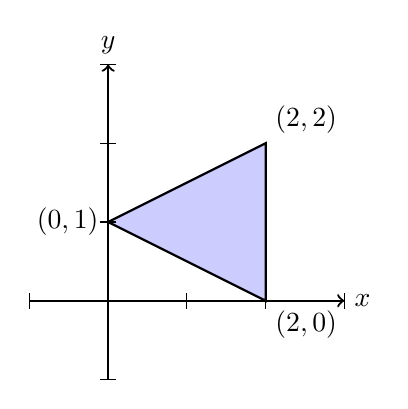
\begin{tikzpicture}[scale=1]
        % Dibujar los ejes coordenados
        \draw[->, thick] (-1, 0) -- (3, 0) node[right] {$x$}; % Eje x
        \draw[->, thick] (0, -1) -- (0, 3) node[above] {$y$}; % Eje y

        % Dibujar el triángulo
        \draw[thick, fill=blue!20] (2, 0) -- (2, 2) -- (0, 1) -- cycle;

        % Etiquetas para los vértices
        \node at (2, 0) [below right] {$(2, 0)$};
        \node at (2, 2) [above right] {$(2, 2)$};
        \node at (0, 1) [left] {$(0, 1)$};

        % Marcas en los ejes (sin números)
        \foreach \x in {-1, 0, 1, 2, 3} {
                \draw (\x, -0.1) -- (\x, 0.1); % Marcas en el eje x
            }
        \foreach \y in {-1, 0, 1, 2, 3} {
                \draw (-0.1, \y) -- (0.1, \y); % Marcas en el eje y
            }
    \end{tikzpicture}
\end{center}